\chapter{Analysis} \label{analysis}
Content of this chapter will focus on defining the problem of pattern matching in the first section, after it the specification of multidimensional arrays will follow, succeeded by the explanation of similarity measures. 

When solving a pattern matching problem there is first needed to specify what is pattern matching which is done in the first section. Then the solution space is explained together with definition of similar measures and their most common types. Fourth section is devoted to introduction of the scientific database SciDB with its binary data format and some possible ways of working with its data.

Fifth section presents multidimensional approximate pattern matching and some of the algorithms solving it. Next part focuses on machine learning methods especially k nearest neighbor and kernel based methods as they can be used for solving or improving of the solution of this problem together with the algorithms presented in the next sections.
\section{Problem specification} \label{spec}
This section will focus on definition of approximate pattern matching. 

First thing first,
the multidimensional array $A$ is composed of dimensions $D$ and attributes $A$ and consists of cells. Dimensions $D$ form the coordinate system for the array. The number of dimensions in an array is the number of coordinates or indices needed to specify an array cell. Each dimension is specified by a unique name, start and end coordinate. Attributes $A$ contain the actual data and are specified by a unique name and value type. This is the base data type used in this work and it is also base representation of data in the SciDB \cite{scidb}. More information about SciDB database can be found in the section \ref{scidb}. Main difference between this model and model used by common relational databases is that this model uses dimensions and attributes whilst relational one uses only attributes.

In the table \ref{tab1} there is an example of the two dimensional array with dimensions: NHL team and Season. Attribute values, in the example number of points acquired during the regular season, are inside the cells, while the dimension values can be seen on the edges. For simplicity reasons only one attribute is considered in this example data. 
\begin{table}
\centering
\begin{tabular} {| c | c | c | c | c | c |}
\cline{2-6}
\multicolumn{1}{c|}{} & \multicolumn{5}{|c|}{Season} \\
\hline
NHL team & 2012--13 & 2013--14 & 2014--15 & 2015--16 & 2016--17\\
\hline
Colorado Avalanche & 39 & 112 & 90 & 82 & 48 \\
\hline
St. Louis Blues & 60 & 111 & 109 & 107 & 99 \\
\hline
Pittsburgh Penguins & 72 & 109 & 98 & 104 & 111 \\
\hline
New York Rangers & 56 & 96 & 113 & 101 & 102 \\
\hline

\end{tabular}
\caption{Example 2D array data structure}
\label{tab1}
\end{table}

Pattern $P$ can be of two types, where the first one is defined as multidimensional array with dimensions $D_p \subseteq D$ and attributes $A_p \subseteq A$ where the number of dimensions $D_p \geq 1$ and number of attributes $A_p \geq 0$.
This type of pattern is called template pattern and it can be used when the user has an exact idea about the result.

And the second type is defined as a condition limiting the values of dimensions and attributes. It consists of a hard constraints in the sense of: Find all parts so that their average value of attribute $A_i$ is lesser than $x$ . This type of pattern is called aggregate pattern, but this type is not used in this work.

As an example of this pattern there can be used the problem of finding weather conditions on earth, which is specified by 2D array with latitude and longitude as dimensions and humidity, wind speed, temperature and other weather related attributes. When in need of finding tornadoes in Europe user would have to use dimensions constraints for Europe and wind and humidity conditions specific for tornado to obtain possible results.

Similarity measure $S$ is a function which quantifies the similarity between two given arrays. 
It is used to compare the pattern and parts of multidimensional array. Which then gives the information about the similarity of the compared parts and the pattern. Its value belongs in the interval $<0, 1>$ where the higher the value the closer the items are, with special case of $1$ which means that the items are exactly the same, and $0$ meaning there is nothing similar between the items measurable by this function. More about similarity measures is in the section \ref{similMeasures}.

Match $M$ is a subset of array $A$ with dimensions $D_m$ and attributes $A_m$, where $A_m \subset A_p$ and the value of similarity measure is higher than a certain threshold.

Approximate pattern matching can then be defined as a function with input parameters of pattern $P$ and multidimensional array $A$ which outputs set of matches $N$ with the use of similarity measures $S$ on arrays.

Exact pattern matching is a special case of approximate pattern matching where the dimensions of pattern $D_p$ are equal to the dimensions of match $D_m$, the attributes $A_m$ are subset of attributes $A_p$ and the value of similarity measure $S = 1$.

Another information about approximate pattern matching and already proposed solutions are explained in the section \ref{multidimApprPattMatch}.

Solutions to this problem are useful and used in every day life for example in: search in database with errors, finding genes, sequence alignment, image registration, computer vision, object recognition, molecular modeling and so on. 

Next chapter focuses on explaining all important terms, algorithms and methods that are commonly used for solving the problem of approximate pattern matching.


\section{Multidimensional array data structure}\label{multidimArrayDataStructure}
Based on \cite{samet} the multidimensional array consists of dimensions and cells in contrary to non dimensional array that consists only of cells. Each cell is composed of attributes. To split these array into grid one can use Regularly gridded chunking where chunks have equal shape and do not overlap or Irregularly gridded chunking which is one of the approaches used by the RasDaMan model \cite{rasdaman}.
To perform selection queries on these arrays there is a need to constraint the query either by dimension or attribute constraint or both of them.

\subsection{Sparse Data}
When data are sparse that means that some attributes can contain 0 or null or empty value. The data can then be viewed as a sparse matrix containing 0 values at the position with no attribute or 0 valued attribute. Because of the nature of this data they offer a big opportunity for using various compressing algorithms to avoid looking through positions with none or 0 values. SciDB \cite{scidb} treats empty cells like they are non existent i.e. they are not evaluated with the count aggregate. Some Linear Algebra operators process them as 0 values and during join, sort and unpack operations they are disregarded.

\subsection{Indexing}\label{indexing}
Indexing improves the speed of data retrieval operation at the cost of additional writes and storage space needed to maintain the index structure. It is used in situations where it is needed to quickly access data without having to search every position. Common methods of indexing are described in the sections below.

\subsubsection{Spatial Indexing}
Spatial indexing can be done four main styles. First of them is by using access methods like point or spatial one, which are used for indexing of B-tree with its variants, Multidimensional range tree, Quadtree, KD-tree and R-trees. \cite{Rtree}. Another choice is to use Space filling curves which is good for maping the space into one dimension, like Peano-Hilbert, Z-order, row-prime order. Fourth choice is for Tilings of the domain space.\cite{joinFractal} This arrays usually have high value locality so the choice is to index individual cels or certain vale ranges as an object. Retrieval of the array indexing of arrays can be done by Depth First Search, but this method is not space efficient. \cite{MDindexingBTree}

When using Quadtree method on of the ways of creating it is to use the Adaptive Mesh Refinement algorithm described below.

\paragraph{Adaptive Mesh Refinement}\label{AMR}
AMR is a function with input parameters of Interval of values, spatial selection and its output is a set of cells with its values. To be returned by the function the cell must satisfy three conditions which are:
\begin{itemize}
\item cell must be uncovered
\item cell belongs to the spatial selection
\item value of the cell belongs in the Interval of values
\end{itemize}
AMR structure is contains of levels and refinement ratio. \cite{AMRindexing} First (coarsest) level is a box (defined by lower and upper corner). Every level can be decomposed into a disjoint union of boxes. A cell contains a pair of information and that is level it belongs to and its position by coordinates. By uncovered it is meant that the cell lies in the last (the least coarse) level. Spatial selection needs to be interpreted within the coordinate system of the first level and a cell in the spatial selection if its coordinates belongs inside the first level selection. Interval of values is simply the interval of values that the elements inside AMR structure can have. Values returned by function are in the pair with structure $<cell, value>$.

Construction of AMR Index tree consists of two phases where in the first one the object is split into boxes which create first level and then in the potential valuable boxes creates another level by splitting the box into smaller ones and so on, if the splitting is needed. In the second phase it creates a tree for every box which is covered by another (smaller) boxes.

\begin{figure}
\centering
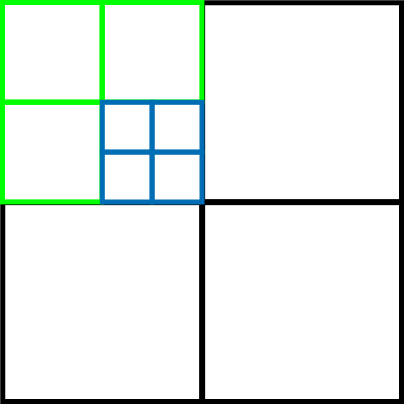
\includegraphics[scale=0.5]{amr_obr.png}
\caption{Example of AMR decomposition, different levels are represented by different colors}
\end{figure}


\subsubsection{Bitmap Indexing}
Bitmap indexing is very useful for its variety. It provides efficient way to evaluate logical conditions on large data sets, because of efficient implementation of the bitwise logical AND, OR and NOT. It also provides significant opportunities for compression (there are also compression algorithms that support compressed domain implementations of the bitwise logical operations and enables query processors to operate directly on compressed bitmaps without the need to decompress). Most of the newer compression algorithms use run-length encoding. Low level bitmaps can be used to index single attribute value and high level ones are used for multiple values. Index structure uses binning strategy which reduces overall number of bitmaps required to index the data, but increases the number of cells later needed to verify. This is called Candidate check. 

This index is useful in cases where the values of a variable repeat very frequently, for example attributes that can have only two values (gender).

Another type of bitmap usage is for Equi-width and Equi-depth binning. Encoding can be performed by:

\begin{description}
\item[Equality encoding:] each bin is encoded by one bitmap
\item[Range encoding: ] each bitmap encodes range of bins
\item[Interval encoding: ] each bitmap encodes $XOR$ of two cells
\end{description}

This can be later compressed by Byte-aligned bitmap code or Word-aligned Hybrid algorithms. 
\subsubsection{Bucket Indexing}
Bucket Indexing methods aggregate data in buckets to save overall size. Data are split into buckets either by having the same or very close index value. Special tree used for storing of this structure is called k-d-b tree and it is a hybrid between k-d tree and B-tree. In its structure one internal node can consist of a set of adjacent regions, leaves can consist of multiple points. It has another variants like LST tree, hB-tree, k-d-b-trie.

\subsubsection{Grid Indexing}
Grid indexing brings it closer to array data model. It splits the domain into non-regularly gridded space and it uses grid file which requires index to maintain linear scale data structure. Algorithm EXCELL creates a modification of grid file allowing it to split the domain space along a single dimension only.

Compressed spatial hierarchical bitmap index \cite{cSHB} creates a spatial hierarchy which consists of nodes, leaves, parents, children, descendants, internal nodes and leaf descendant of a node. The structure itself creates a set of bitmaps where for each node there is a corresponding bitmap and then it creates and stores compressed bitmap for each node, except empty ones which all have one node. This method has one input parameter and it is target block size. Algorithm then ensures that all index files written to the disk are at least block size big which is done by concatenation of compressed bitmap files. This means that the size of the files will be upper bounded while the cost of the bitmap reads will be lower bounded.

\subsubsection{Inverted Indexing}
Unlike common indexing methods (mentioned above) this methods goal is to create a set of all unique values in the data where each value has a list of the documents containing it. This solutions is mainly used for databases containing text to allow full text searches. However the drawback of this method is in a high processing cost of a newly added elements. \cite{invertIndex}

\subsubsection{Medial Axis Transformation}
Before defining Medial Axis Transformation (MAT) there is first needed to explain what a \textit{disk} is.
Disk is some specified shape or neighbourhood of some specific point and it also has a radii, it belongs in the object and can not reach out of the object bounds. Object can then be defined as the union of the maximal disks it contains.

Medial axis transform of S consists of the centres of these disks together with their radii. The distance of a point x in S from S is then the length of the shortest path from x to the complement S. MAT can also be defined as the set of all points in S which do not belong to the minimal path of any other point, together with their distances. This can be imagined like constitution of a skeleton.

Each object is then defined by the triple $(c, d_c, w_c)$ where $c$ is the cell, $s_c$ is the largest square in which it is contained with width $w_c$. Set of these triples is called MAT of object S. This is very compact method for simple shapes.

In the field of digital pictures disks are approximated by squares and their orientation depend on the definition of grid distance, which also defines the type of the skeleton.

\begin{figure}
\centering
\begin{subfigure}[t]{.48\textwidth}
 \centering
 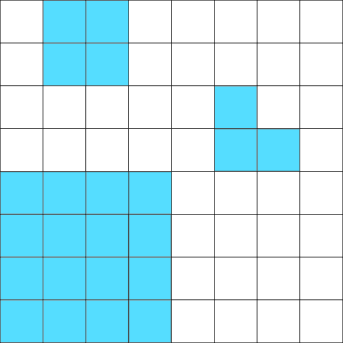
\includegraphics[width=.8\linewidth]{MAT_todo.png}
  \caption{Objects and cells that MAT algorithm will be performed at}
  \label{fig:sub1}
\end{subfigure}%
\hfill%
\begin{subfigure}[t]{.48\textwidth}
 \centering
 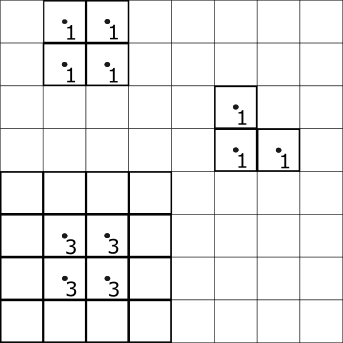
\includegraphics[width=.8\linewidth]{MAT_done.png}
 \caption{MAT for the collection of objects and cells, maximal block is anchored at the unit-size element at its center}
\end{subfigure}
\end{figure}

Base types of distances that can be used are:
\begin{itemize}
\item Chess-board distance - disks are upright squares
\item city block distance - disks are approximation of diagonal squares
\item Euclidean distance - disks are discs, also more appropriate in continuous space
\item Absolute value distance - disks are diamonds
\end{itemize}

When using irregular grid it can decompose the space using hyperplanes resulting in collection of blocks. By this there can be recreated irregular block sized grid, where no recursion is involved and block decomposition is handled by explicit representation. These blocks are not congruent (this will add access structure containing linear scales which indicates position of partitioning hyperplane).

Representation of block decomposition can be done by using different types of quadtree or octree (\ref{octree2}). Most commonly used decompositions are:
\begin{itemize}
\item Multicoloured quadtree - can contain more than two colours and also more block labels
\item Binary quadtree - for black and white values only
\item Block specified by a pair of coordinates - specified by upper left corner coordinate and size of the side
\item Morton block - encoded by localization code (variant of Morton number), which is power of two and Morton ordering is NW, NE, SW, SE
\item Scan of resulting representation from extreme right end to first zero valued bit
\item Sorting the values in increasing order - Efficient pixel interleaving compression technique (EPICT)
\end{itemize}

\begin{figure}
\centering
\begin{subfigure}[t]{.48\textwidth}
 \centering
 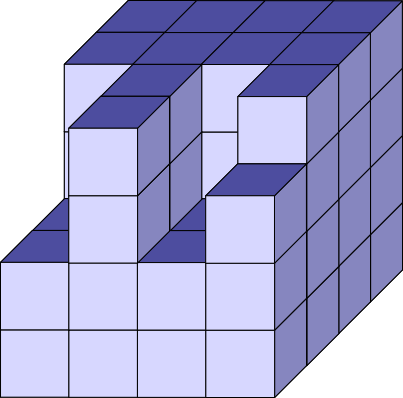
\includegraphics[width=.8\linewidth]{mat3d_todo}
  \caption{Object that block decomposition will be used on}
  \label{fig:sub1}
\end{subfigure}%
\hfill%
\begin{subfigure}[t]{.48\textwidth}
 \centering
 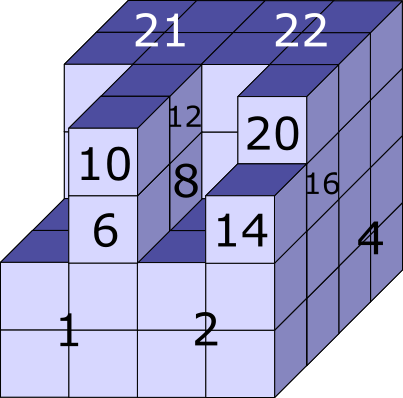
\includegraphics[width=0.8\textwidth]{mat3d_todo_other2}
 \caption{Region octree block decomposition of the picture above}
\end{subfigure}

\vspace{10px}
\begin{subfigure}{\textwidth}
\centering
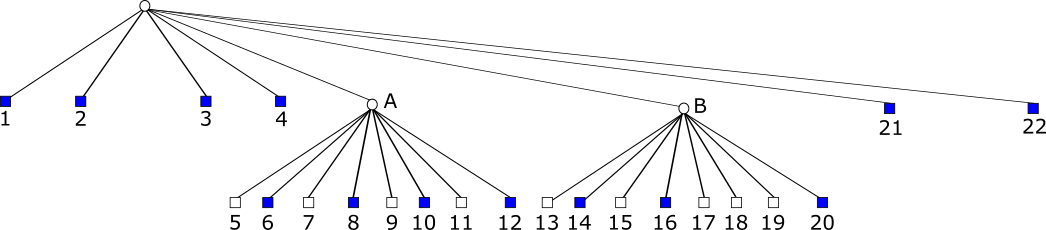
\includegraphics[width=\textwidth]{mat3d_strom}
\caption{Octree block decomposition of the picture in Figure 1}
\end{subfigure}
\caption{Example of octree decomposition.}
\label{octree2}
\end{figure}

%\begin{figure}
%\centering
%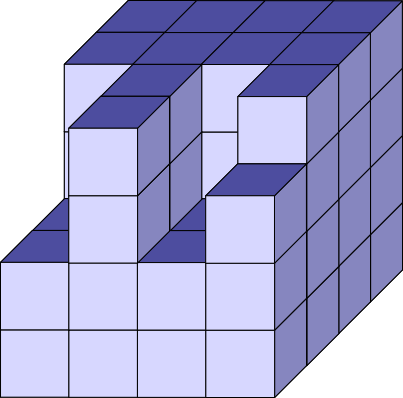
\includegraphics[scale=0.5]{mat3d_todo.png}
%\caption{Object that block decomposition will be used on}
%\end{figure}
%\begin{figure}
%\centering
%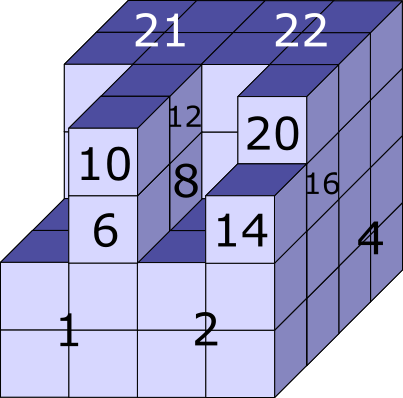
\includegraphics[scale=0.5]{mat3d_todo_other2.png}
%\caption{Region octree block decomposition of the picture above}
%\end{figure}

%\begin{figure}
%\centering
%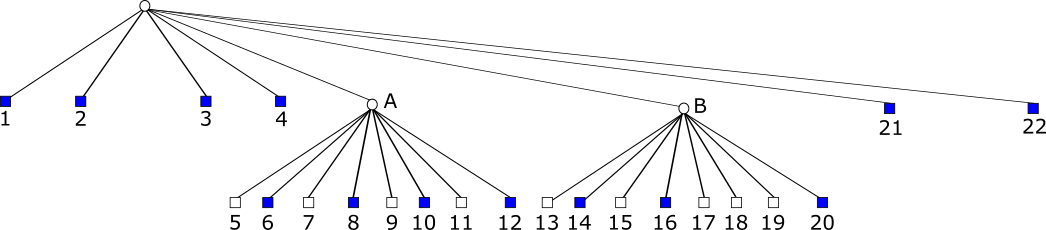
\includegraphics[width=\textwidth]{mat3d_strom.png}
%\caption{Octree block decomposition of the picture in Figure 1}
%\end{figure}
For more informations about typical usage and types of MAT see \ref{appendixMAT}.


\subsection{Representation of multidimensional data}\label{represOfMultidimData}
When representing hierarchical domains there are three categories of different approaches.

First approach is that there can be used the $K^n-treap$ which is an extension of $k^2-treap$ and it uses $k^n-tree$ to store its topology. It is an efficient representation of wide empty areas which splits each dimension into k equal sized parts and saves it as a structure of values and tree structure. It can be searched from root to leaves for aggregated values of a range cells using the depth-first multi-branch traversal.

Second representation is per CMHD which means Compact representation of Multidimensional data on Hierarchical Domains. This algorithm recursively divide matrix into several submatrices. It assumes same height of all the hierarchies. If needed of artificial levels they can be added by subdividing all the elements of a level in just element (itself).

Third possibility is to use Queries where elements of the different dimensions are all on the same level in their hierarchies. Different levels contain different labels. It is required to have top down traversal when searching hash tables for labels provided by the query for different dimensions to locate corresponding nodes. From nodes it traverse each hierarchy upwards to find out its depth and child that must be followed to reach it. \cite{efficientRepre}
\section{Similarity hashing}\label{similHashing}
Hashing approach is based on transforming the data item into a low-dimensional representation, or a short code composed of a sequence of bits.

This method is used to hash similar items into the same buckets, it is used in similarity searching systems. To measure similarity a feature based distance can be used. When hashing data it is the same approach as transforming them into a low dimensional space. Specific hashing approaches used in implementation will be explained in the section Implementation.

Outcomes of this approach can be used in nearest neighbour search problem.

\subsection{Locality Sensitive Hashing}\label{LSH}
This method was proposed in 1998 for approximate nearest neighbour search in high dimensional spaces. Research often views this method as: \textit{``probabilistic similarity-preserving dimensionality reduction method from where the hash codes can provide estimations to some pairwise distance or similarity''}  \cite{hashing}. The essential idea of this approach is to have a hash function that will return the same value for nearby items from the data. But to achieve high precision, there are several disadvantages. First of them is that to acquire wanted precision the usage of long hash codes is needed, which reduces the recall. This can be solved by creating multiple hash tables but it also increases storage requirements as well as the query time. Second obstacle is that LSH can be applied only in certain metrics e.g. $l_p$ and Jaccard. 

Main usage of this approach is in finding near-duplicate web pages, image detection, clustering and so on. 

Types of this method can be split into several categories.
First of them is based on the $l_p$ distance: LSH with $p$-stable distributions, Leech lattice, Spherical LSH, Beyond LSH.
Another type is split by the usage of Angle-Based distance: Random projection, Super-bit LSH, Kernel LSH, LSH with learned metric, Concomitant LSH, Hyperplane hashing.
Next type of Locality Sensitive Hashing is based on Hamming distance. There are also types dependent on Jaccard coefficient: Min-hash, K-min sketch, Min-max hash, B-bit minwise hashing, Sim-min-hash.
Among other similarities hashes belongs: Rank similarity, Shift invariant kernels, Non-metric distance, Arbitrary distance measures.
Usability of this method highly depends on the quality of hashing method used.
\subsection{Learning to Hash}
Goal of this method is to learn dependencies in the data and create task-specific hash function that gives compact binary codes to achieve good search accuracy. \cite{learnHash} For achieving of this goal several sophisticated machine learning tool and algorithms have been adapted to hash functions design. Among the most important belong: boosting algorithm, distance metric learning, asymmetric binary embedding, kernel methods, compressed sensing, maximum margin learning, sequential learning, clustering analysis, semi-supervised learning, supervised learning, graph learning, ....

This concept can be used for solving of hashing-based ANN search.

\subsection{Randomized Hashing}
This type of hashing covers e.g. the LSH family and has been popular due to its simplicity. There are two main types of this approach based on the problem solution space. 

First of them is the Random Projection Based Hashing which is based on an idea of preserving the locality in the original Hamming space.

In machine learning, recent research is focused on leveraging data-dependent and task-specific information for improving efficiency of hash functions like this. Some of the examples are: using kernel learning with LSH \cite{kernelLSH}, boosted LSH \cite{boostLSH} and non-metric LSH \cite{nonMLSH}.

Second type is hashing based on random permutations. This method is also known as min-wise independent permutation hashing or MinHash. Originaly the Minhash was applied in clustering and for eliminating of near-duplicates among web documents represented as sets of the words. \cite{minhashuse}

\subsection{Data-Dependent and Data-Independent Hashing}
This category of hashing is based on the knowledge about the given dataset. Randomized hashing mentioned in previous section belongs in the category of data-independent hashing as it does not need any special information about the dataset. However this is also a limitation of this approach as these methods have strict performance guarantees and they are not specifically designed for certain datasets. Limitations of this approach gave birth to data-dependent approach which uses supervision to design better and more efficient hashes. \cite{learnHash} 

\subsection{Supervision Hashing}
This method can be split into three more categories based on the level of supervision.

First of them is unsupervised which methods try to integrate data properties like distribution into the hash value. Examples of this approach are: 
\begin{itemize}
\item Spectral Hashing -- idea of this hashing is to hash similarity based on Hamming distance and use only a small number of hash bits
\item Graph Hashing -- this method revolves about hashing graphs e.i. nodes and edges
\item Kernelized LSH -- this approach is focused on using kernel functions as a hashing functions
\item Spherical Hashing -- basic idea is to use a hypersphere to formulate a spherical hash function
\end{itemize}

Second is supervised learning which ranges from usage of kernel methods and metrics (defined in section \ref{similMeasures}) to deep learning. Examples of this approach are introduced in papers \cite{LM1} and 
\cite{LM2}.

Last type using semi-supervised learning usually designs hash functions based on both labelled and unlabelled data.

Categories above can again be divided into point-wise, pair-wise, triplet-wise and list-wise subcategories. This hashes can be created either by using information from a single item or an arbitrary number of items \cite{learnHash}.

\subsection{Linear and Nonlinear Hashes}
This type is based on the type of function used to create hashes, e.g. when using linear function for hash creation it is linear hash, and vice versa. Because of the computational requirements linear functions are usually used more often than non-linear ones. \cite{learnHash}

\subsection{Weighted Hashing}
When using traditional hashing the goal is to map the data into \textit{non-weighted} Hamming space. However sometimes it can be easily observed that different bits are behaving differently \cite{learnHash}. Because of this a technique were designed that learns a specific weight for each bit of the original hash.

\section{Similarity measures}\label{similMeasures}
By using a term similarity there is meant measure of how "close" to each other two instances are by quantifying the dependency between two sequences. The closer they are the larger the similarity value. However there are two ways of approaching the similarity measure. First of them is dissimilarity, which is a measure of how different two instances are. Dissimilarity is larger the more different the instances are. Some scientists use word proximity by which they refer to either similarity or dissimilarity.

Similarity can be measured between strings, numbers, tuples, objects, images and so on, and its value is normalizes, which means in the interval [0,1], where 1 is for exact match and 0 for completely different objects. \cite{simDissim}

A similarity measure M is considered a metric if its value increases as the dependency between corresponding values in the sequence. A metric similarity must satisfy following conditions:
\begin{itemize}
\item Limited Range: $M(X,Y) \leq S_0$ for some arbitrarily large number $S_0$
\item Reflexivity: $M(X,Y) = S_0$ if and only if $X=Y$
\item Symmetry: $M(X,Y)=M(Y,X)$
\item Triangle Inequality: $M(X,Y)M(Y,Z)\leq [Z(X,Y)+M(Y,Z)]M(X,Z)$
\end{itemize}
Where $S_0$ is the largest similarity measure between all possible X and Y sequences.

In a similar way a dissimilarity measure D is considered a metric if it produces a higher value as corresponding values in X and Y become less dependent. A metric dissimilarity must satisfy following conditions:
\begin{itemize}
\item Non-negativity: $D(X,Y) \geq 0$
\item Reflexivity: $D(X,Y) = 0$ if and only if $X = Y$
\item Symmetry: $D(X,Y) = D(Y,X)$
\item Triangle Inequality: $D(X,Y) + D(Y,Z) \geq D(X,Z)$
\end{itemize}

Typically, if presented with a similarity measure, it is revertible into dissimilarity measure and vice versa.

Generally there is a request for measures to have properties of a metric but they can be quite effective even without being a metric. For example, ordinal measures are not metrics but they are very effective in comparing images captured under different lighting conditions.\cite{simMeasuresLecture}

Similarity measures can be divided into five main categories depending on their domain or character. In the following sections all these categories will be described and their main methods mentioned.

For more informations about similarity measures see: \cite{clusteringSimMeasure} \cite{simDissim} \cite{simMeasuresLecture}.

\subsection{Numeric methods}
This methods can be used for numeric attributes where it can be treated as a vector $\bar{x}=(x_1,...,x_N)$ for attributes numbered $1,...,N$. One of the most commonly used methods are shown in the list below as described in \cite{simvzorecky}.
\begin{itemize}
\item Euclidean Distance: $d_E (\bar{x},\bar{y})=\sqrt[2]{\sum_{k=1}^N (x_k-y_k)^2} $
\item Squared Euclidean Distance: $d_E (\bar{x},\bar{y})=\sum_{k=1}^N (x_k-y_k)^2 $
\item Manhattan Distance: $d_M (\bar{x},\bar{y})=\sum_{k=1}^N 
{\lvert x_k-y_k \rvert}$
\item Minkowski Distance: $d_{M,\lambda} (\bar{x},\bar{y})=(\sum_{k=1}^N (x_k-y_k)^\lambda)^{\frac{1}{\lambda}} $
\item Chebyshev Distance: $d_{M,\inf} (\bar{x},\bar{y})=max_{k=1,...,N}(\lvert x_k-y_k \rvert) $
\item Earth Mover's Distance: $d_{EMD}(P,Q)=\frac{\sum_{i=1}^m\sum_{j=1}^n f_{ij}d_{ij}}{\sum_{i=1}^m\sum_{j=1}^n f_{ij}}$, where $P$ has $m$ clusters with $P={(p_1, w_{p1}), (p_2, w_{p2}),...,(p_m, w_{pm})}$ where $p_i$ is the cluster representative and $w_{pi}$ is the weight of the cluster. Similarly signature $Q={(q_1, w_{q1}), (q_2, w_{q2}),...,(q_n, w_{qn})}$ has $n$ clusters. $D=[d_{ij}]$ is the distance between clusters $p_i$ and $q_j$. $F=[f_{ij}]$ is the flow that minimizes the overall cost.
\end{itemize}

\subsection{Edit-Based methods}
First it is needed to define exact and truncated match. Similarity of exact match is equal to 1 if x=y and zero otherwise. Similarity of truncated match from the beginning is 1 if $x[1:k] = y[1:k]$ and zero if $x[1:k] \neq y[1:k]$, also the similarity of the end of the truncated match is 1 if $x[k:n] = y[k:n]$ and zero if $x[k:n] \neq y[k:n]$. And the similarity of encoded object is 1 if $encode(x)=encode(y)$ and 0 if $encode(x) \neq encode (y)$. \cite{sim2Dstrings}
\subsubsection{Hamming distance}
Hamming distance is defined as the number of positions in which two equal length strings differ. It can be understand as minimum number of substitutions needed to change one string into another or minimum number of errors that could transform one string into the other.
This method is used mostly for binary numbers and to measure communication errors. When used within binary numbers it can be counted as number of 1s in XOR of the numbers. \cite{hamming}

For example the Hamming distance of strings ABC and CBA is 2 as only 1 character matches and 2 would need to be substituted.

\subsubsection{Edit distance}
Edit distance can be understand as minimal number of edits required to transform one string into the other. This method compares strings based on individual characters. As valid edit steps there are counted Insert, Delete and Replace operation, where each edit has cost 1. Also as an alternative the smallest edit cost can be counted. Its script is based on dynamic programming algorithm. This distance can also be known as Levenshtein distance. \cite{editDist}

Edit distance of strings ABC and CBA is 2 as 2 positions would need to be edited.
\subsection{Token-Based methods}
Main idea of this method is that every object can be separated into tokens using some kind of a separator. For example space, hyphen, punctuation or special character can be used as a separator in strings. Which is also a problem of this algorithm as lot of both hyphenated and non-hyphenated words are common, the same as words with apostrophes, numbers or periods. Another solution is to split strings into shorter sub-strings of length n and thus creating n-grams. \cite{tokenDist}

\subsection{Hybrid methods}
Hybrid methods are usually combination of some of previously mentioned methods as presented in \cite{hybrmeasure}.

\subsubsection{Monge-Elkan}
Monge and Elkan proposed this simple but effective method for measuring the similarity between two strings containing multiple tokens with the use of internal similarity function capable of measuring the similarity between two tokens a and b. 
Imagine two texts A and B with their respective number of tokens $\lvert A \rvert$ and $\lvert B\rvert$. 
The algorithm measures the average similarity of the values between pairs of more similar tokens within texts A and B. 
The formula is: 
$ME(A,B)=\frac{1}{\lvert A \rvert} \sum_{i=1}^{\lvert A \rvert} max (sim(A_i, B_j))_{i=1}^{\lvert B\rvert}$, where $sim(a, b)$ is internal similarity function.
\subsubsection{Extended Jaccard Similarity}
If strings contain multiple words then choose words as tokens and use internal similarity function to calculate similarity between sets of tokens as the ratio of the number of shared attributes (AND operator) and the number possessed by OR operator.
\subsubsection{Tf-idf}
Term frequency (tf) weight measures importance of term in a document and inverse document frequency (idf) measures importance in collection (this reflects the amount of information carried by the document). These two measures are then multiplied with some heuristic modifications.

\subsection{Similarity measures on arrays}
When measuring a similarity in 2D array one can use Aho-Corasick's multi-string searching algorithm \cite{ahocor} which uses a finite automaton or there can be used an algorithm by Baeza-Yates and R{\' e}gnier \cite{baeza1993fast} which uses Aho-Corasick's algorithm in every row and Knuth-Morris-Pratt algorithm on every column, searching for the row indices of the pattern. If there is only one pattern to search for there exists optimal algorithm from K{\"a}rkk{\"a}inen and Ukkonen who improved an algorithm from Baeza-Yates and R{\' e}gnier so it achieves $O(n^2 \log_\sigma (m) / m^2)$ where $\sigma$ is the size of an alphabet, $n$ is the size of a text and $m$ is the length of a pattern \cite{karkoptimal}. 

On the other hand, when searching for higher number of patterns (thousands) in one string and allowing maximum of one mistake Muth and Manber proposed a solution in \cite{1erroronly}.

If tasked with probabilistic 2D pattern matching algorithms are proposed by \cite{kr87} but running time ($O(n^2)$) makes it unusable in practice. Its improvement was introduced by \cite{zt89} where are two versions, one using Knuth-Morris-Pratt algorithm and second with a variant of the Boyer-Moore algorithm.

If the pattern can be scaled (i.e pattern of a picture appears at a different size), there can be used the work of \cite{realscaledmatch} and \cite{alphscalematch}. And if it can be rotated some important studies are: \cite{patternrotation1,patternrotation2,patternrotation3}.


\begin{figure}
\centering
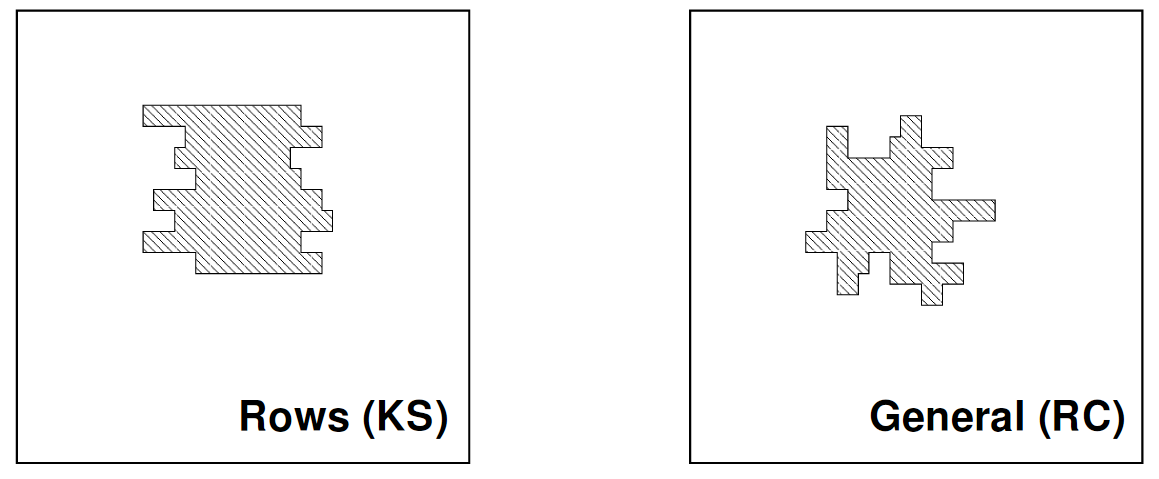
\includegraphics[scale=0.3]{RC_KS.png}
\caption{KS and RC error models \cite{mdApproxPM}}
\label{ks_rc}
\end{figure}


\subsubsection{KS}\label{ks}
Krithivasan and Sitalakshmi (KS) defined the edit distance in two dimensions as the sum of the edit distance of the corresponding row images. Using this model they search a subimage of size $m \times m$ into a large image of size $n \times n$ using a generalization of the classical one-dimensional edit distance algorithm.
The KS model can be extended into more than two dimensions, but it allows errors along one of the dimensions only. \cite{mdApproxPM}
An example can be seen in the figure \ref{ks_rc}.
\subsubsection{R,C}
In this model, each row (column) is treated as a single string which is compared to other rows using the one-dimensional edit distance, but 
whole rows can be inserted and deleted as well.
Generalization of R,C model is RC model where errors can occur along rows or columns at any time. This model is much more robust and useful for more applications. Example of the RC model is in the figure \ref{ks_rc}. \cite{mdApproxPM}
\subsubsection{L}
If it is needed to change both the row and column at the same time (for example when scaling) there could be used the L-shape for decomposition of the subimage and thus have the same extensions for rows and columns. When comparing L-shapes they are seen as two one-dimensional strings. L-shape string consists of the first (left) $j$ elements of the \textit{i}-th row and the first (top) $i-1$ elements of the \textit{j}-th column.

This idea was first presented by Raffaele Giancarlo \cite{lshape} where it is used for building of Lsuffix tree with the use of Lstrings which can only be used for square matrices of text. Giancarlo divides the application of his solution into two sections: dictionary matching algorithms and pattern retrieval algorithms.

\subsubsection{All}
This model uses both decompositions at the same time (RC and L) computing the minimal value of all possible cases. It
is easy to show that $KS(A,B) \geq R(A,B) \geq RC(A,B) \geq All(A,B)$ and that $L(A,B) \geq All(A,B) $ because each case is a subset of the next. On the other hand, there are cases where $RC(A,B)$ will be less than $L(A,B)$ and vice versa. \cite{mdApproxPM}


\subsubsection{Vector space model}
This is an algebraic model using vectors as representation instead of arrays. It is commonly used for handling of text documents in the situations like information filtering, information retrieval and indexing.

The procedure of this model can be split into three stages. First phase is document indexing when the words that do not describe the content are removed (in English words like: the, is) so the document will be represented only by words bearing content. Second phase is term weighting which is based entirely on single term statistics. Term weighting has three main factors and that is: term frequency factor, collection frequency and length normalization factor. These factors are then multiplied together to make the resulting weight. Third stage is the final computation of similarity coefficient which is usually determined by the cosine coefficient by measuring the angle between the document vector and the query vector. Other usable measures can be Jaccard and Dice coefficient.

\subsection{Domain-Dependent}
Among some special similarity measures belong methods processing only one specific domain and thus the name domain-dependent measures.
Widely used methods for handling this problem can be divided into categories based on the field like for example: phonetic methods, time and space methods, numerical comparison and binary vectors. 

Analysis of two examples is given in the sections below but this work will focus mainly on commonly used measures for arrays. However if the data for these measures are correctly preprocessed they can be used on arrays.

\subsubsection{Time and space comparison}
This is a very wide field of work mainly because the diversity of categorical data one can use for clustering, classification or any other case in need of some distance measure.
To get similarity of time and space objects numerical methods are used to calculate differences in days. In other cases data can be converted (dates of birth into age) and then relevant methods can be used on this new attributes.
When approached with geographic locations its similarity is estimated by using the great circle distance which is the shortest distance between two points along the great circle that contains both points. Popular method to compute the great circle distance is the Haversine formula.
Time series data such as EEG there is a method for choosing a time interval and compare values of both the time series after the lapse of each interval. This has a several drawbacks because of the fixed interval if the series get out of sync this method can result in exaggerated distance estimates. To avoid this problem there is possible use of Dynamic Time Warping method which is robust enough to speed variations and computes more realistic distance estimate by using recursive formulation.
In the list below there are measures useful for categorical data:
\begin{itemize}
\item Overlap - Measures number of attributes that match both data instances. Its range is $[0,1]$ with 0 occurring when there is no match and vice versa.
\item Goodall - Attempts to normalize the similarity between two objects. Assigns higher value to a match which is less frequent and then tries to combine similarities based on attribute dependencies. This is very computationally expensive.
\item Gambaryan - gives higher value to matches closer to being half similar. The measure is close to Shannon entropy. 
\item Eskin - Measure assigns higher value to mismatches from attributes with many values.
\item Inverse Occurrence Frequency (IOF) - Assigns lower value to mismatches on values with higher frequency. In contrary to inverse document frequency it is computed not on binary matrix but directly on categorical data.
\item Occurrence Frequency - Uses opposite weighting compared with IOF (i.e. less frequent mismatches are given lower value)
\item Burnaby - Assign low value to mismatches on rare values and vice versa. This method is based on arguments from information theory.
\item Lin - Assign higher weight to matches on frequent values and conversely with lower values.
\item Smirnov - This measure is based on probability theory based on value's frequency but also the distribution of other values. It means that the value is high for a low frequency of matches and vice versa.
\item Anderberg - Assign higher similarity to rare matches, because they should be more important, and low similarity to rare mismatches. This measure cannot be written in equation form.

\end{itemize}

%\subsubsection{Binary vectors}
%Simple Matching Distance or Simple weighted Matching Distance can be counted for symmetric binary attributes (i.e. both 0 and 1 values have equal importance).
%When having asymmetric attributes possibilities are: Jaccard distance, Weighted Jaccard distance, Non-binary categorical attributes and Simple Matching distance.
%To fully understand binary classification there is a need of explaining what a confusion matrix is. A confusion matrix is a table used to describe the performance of a classification model on a data the true values are known. Ranges of the table is usually 2x2 (for two classes) and in the upper left corner there is a true positive value which signifies how many values are correctly classified as the first class. In contrary in the bottom right corner there is a number of true negative values, i.e. values that are correctly clasified as second class. In the upper right corner there is a number of falsely classified positive values hence false positive and similarly in the bottom left corner there is a number of falsely classified negative values hence false negative.



\section{SciDB}\label{scidb}
Nonexistence of usable scientific database gave birth to the SciDB. It was created to fulfill requirements given by scientists. Between the main requirements was to be able to contain multi-petabyte amounts of data, the preponderance of the data to be arrays, to be able to perform complex analytics, to have open source code, data can never be overwritten, it needs to be able to do provenance (trace backward), must work with uncertainty (because data comes with error bars) and must implement version control. This system was developed in C++ and supports Linux systems.

\subsection{Data model}

Because of these requirements the native data model chosen was array data where objects are N-dimensional array and not tables. Arrays with integer dimensions are divided into storage chunks which are composed of a stride in each dimension. Also, arrays are uniform, which means that all cells in a given array have the same collection of values. \cite{scidb}

This database supports schema migration, so attributes can be promoted to dimensions and dimensions can be deprecated to attributes. These operations can be performed by the transform command which pushes all dimension values up one to make a slot for new data. It can also reshape and array, flip dimensions for attributes and transform one or more dimensions into polar coordinates.

\subsection{Language}

SciDB was developed to work with functional and SQL-like query language. The functional language is called AFL (array functional language) and the SQL-like is called AQL (array query language) and is then compiled into AFL. Array query language has SQL like construction and is able to compute linear algebra queries. It also contains loose coupling model for analytics which in this case is ScaLAPACK running alongside SciDB performing matrix operations.

\subsection{Data storage}
Arrays are stored on disk in fixed-sized chunks with extra storage chunks where the "not valid" cells are. These chunks are heavily encoded. Chunks are distributed with the use of hashing, range partitioning or a block-cyclic algorithm. It is usually a two level chunk/tile scheme where chunks are split into tiles. The chunking strategy is supporting multidimensional queries in a straightforward way i.e. chunking automatically provides an index, however this suffers from skew problems (e.g. think of density of people living in Manhattan and village). This problem can be solved by creating super-chunks from sparse chunks or by creating variable sized chunks. Because of this the database supports arbitrary number of splits to keep the chunk size below the threshold.

Because of the need to never discard data even when wrong the storage strategy was chosen as no overwrite. There is special dimension for each array version. This is managed by special integer counter which begins at zero and increases with each update until array is destroyed. Need to trace backwards is arranged by backwards deltas which contains a chain of references to previous versions. When in need of inserting and updating certain cell the database will put new values at the appropriate version in the array while delete operation will simply put "not valid" label to the cell. Version can be tied to wall-clock or special version names.

Design of the stored data was created as shared nothing which enables running local query in parallel across some collection of nodes followed by scatter-gather data shuffle to rearrange data for the next collection of local operations. But chunks can overlap by a user specified amount to support parallel execution of nearest neighbour, feature detection and so on.

Specification of binary file format used for chunk storage is given in the appendix \ref{binForm}.

\subsection{Query processing}

Query processing is constrained by three tenets.
First of them is to aim for parallelism in all operations with as little data movement as possible. SciDB is fundamentally focused on providing the best response time for AQL which can be helped by redistributing data. It tries to optimize the query parse tree by examining the operations that commute (cheaper of them are pushed down the tree) and examining blocking operations. This operations requires redistribution or cannot be pipelined from the previous operation which means they require a temporary array to be constructed.
Second tenet is that incremental optimizers have more accurate size information and can use this to construct better query plans. Optimizer in this case is incremental and it picks the best choice for the first sub-tree to execute and not until it is done it chooses the second sub-tree and so on.
Third tenet is to use a cost-based optimizer. SciDB tries to perform simple cost based plan evaluations but it plans only sub-trees. The optimizer provides these steps until there are no more sub-plans: choose and optimize next sub-plan, reshuffle data if required, execute a sub-plan in parallel on a collection of local nodes and collect size information from each local node.

As to the provenance task. The database admin is allowed to specify exact amount of space he is willing to allocate for the provenance data. \cite{scidbarch}

\subsection{Use case}

Between most common use cases of this database belong satellite imagery, astronomy applications, genomics and commercial applications.

Everyone can create their own queries because this database supports user defined data types and functions, but with specified amount of overlap. It can also work with uncertain cell values, but not uncertain dimensions and in-situ data, so you can use SciDB without loading your data.

\subsection{ArrayLoop System}
ArrayLoop is a middle-ware system that translates queries expressed in the model into queries executable by the SciDB. It uses iterative array model, which means there is an array being modified during iteration. Termination condition of this function is represented as an AQL function. This model is interested in major steps that can be decomposed into a minor ones which gives us possibility of parallel evaluation. By major steps its meant that function operates on all cells in array and minor step is otherwise. First of all there is need to assign what to do which is done by \textit{Pi} function. Then it is needed to compute aggregate function separately for each group.  This computation can be done with the help of an algorithm presented in \cite{marginals} and described in the section below \ref{marginals}. After that the records are updated with the new values and this generates new subset containing the results.
For best usage of this algorithm was developed FixPoint function where user specifies the logic of iterative algorithm and it will translate it into ArrayLoop which prepares it into AQL and then SciDB can finally process it.

To transform the function into the AQL format, ArrayLoop first automatically expands and rewrites the operation into an incremental implementation, if it is possible, and efficiently computes the last state of iterative array with the use of the updated cell in each iteration. Then it extracts (for each array chunk) the overlap area of neighbouring chunks and stores this overlaps together with the original chunk which provides both the core and overlap data to the operator during processing. In the final step it identifies outlines of the structures on a low resolution array and then refines details onto high resolution arrays. \cite{arrayloop}

\subsubsection{Computing marginals} \label{marginals}
As a marginal of a data cube it can be understood the aggregation of the data in all those tuples that have fixed values in a subset of the dimensions of the cube. Order of the marginal is the number of dimensions over which aggregation is happening. Mapping of reducers q and replication rate r is that no reducer associated with more than q inputs and for every output there is some reducer that is associated with all the inputs that output needs for its computation. Dimensions in this case have same number of different values.
Function C(n,m,k) defines minimum number of sets of size m out of n elements that every set of k out of the same n elements is contained in one of the sets of size m, and it is called the covering number.
Different sets of n,m,k are handled differently but when approached with unknown values it can be solved as: one group of handles contains dimensions to m-k+1 plus any k-1 dimensions from group 2, and others are formed recursively to cover the dimensions of group 2 and have none of the members of group 1.
This problem can be generalized as a problem with weights of dimensions and dividing dimensions into several groups. \cite{marginals}

Example of computing marginal in three dimensional space (as seen in the pictures \ref{margin1} and \ref{margin2}):\\
SELECT SUM(V) \\
FROM DataCube \\
WHERE D1 = x, D2 = y, D3 = z;\\
\begin{figure}
\centering
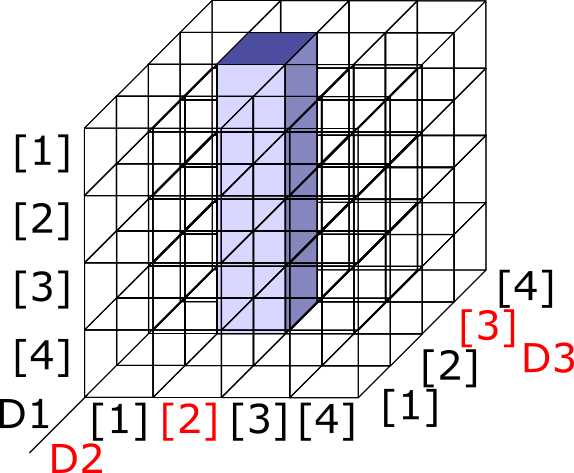
\includegraphics[scale=0.5]{marg1d.png}
\caption{Example of DataCube and selecting dimensions where y=2 and z=3}
\label{margin1}
\end{figure}
\begin{figure}
\centering
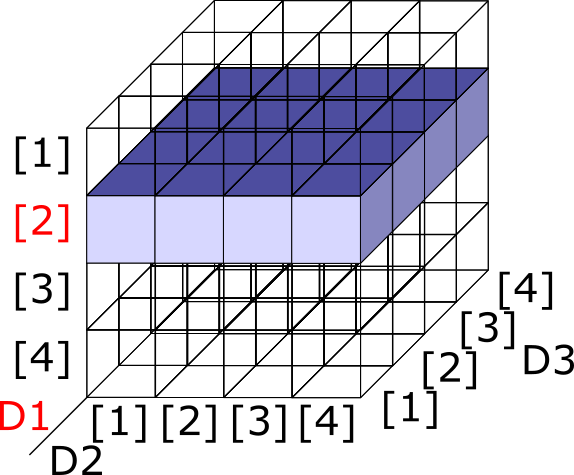
\includegraphics[scale=0.5]{marg2d.png}
\caption{Example of DataCube and selecting dimensions where x=2}
\label{margin2}
\end{figure}


\subsection{Window aggregation}
Window aggregate executes aggregate operators over a sliding window (sub-array), as seen in the picture \ref{windowAMwin}. It has five types of operators: min, max, sum, average and percentile.
Its computation scheme is incremental and has two stages. It tries to maintain intermediate aggregate results of the current area and reuse them. Inside the staged it moves basic window in the first N-1 dimensions, then it moves the window along with the last dimension and incrementally compute the aggregate result for each window. After all windows derived from the basic one are processed it is completed and it returns to the first step until all computation rounds of the basic windows are processed.

\begin{figure}
\centering
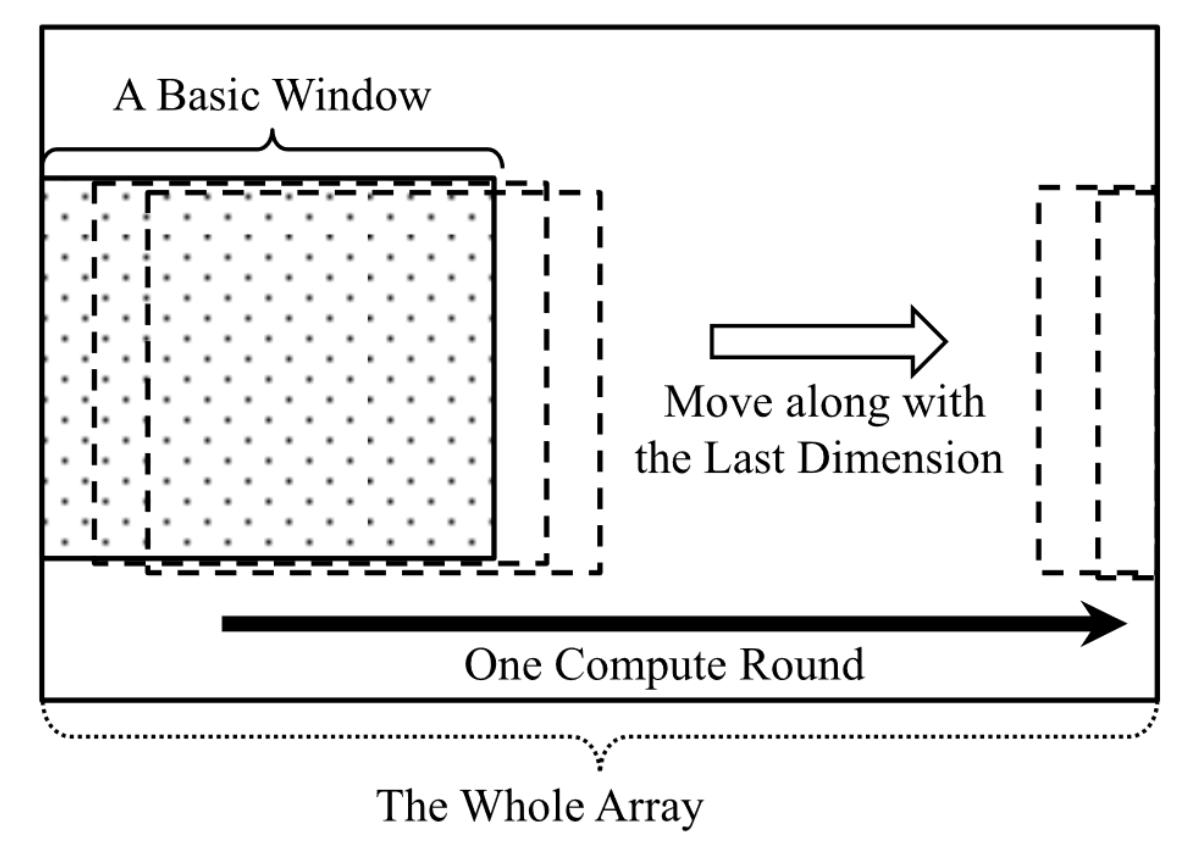
\includegraphics[width=0.6\textwidth]{windowAM.PNG}
\caption{Example of a sliding window \cite{windowAggr}. }
\label{windowAMwin}
\end{figure}

Sum and average operators are very similar as average uses sum and divides it by number of the elements. Because of this there will be only sum operator explained. This operator reuses SUM computed in previous windows by creating list structure (SUM-list) which contains sum values of every window unit. It generates basic window, computes its sum and initialize sum-list. Then it moves the window along with the last dimension with one step on one window unit, scans it and calculates the sum and updates the sum-list. Then it proceeds forward and continue to move the basic window down to obtain new ones. An example of creating and moving the SUM window can be seen in the pictures \ref{windowAM1} and \ref{windowAM2}.

\begin{figure}
\centering
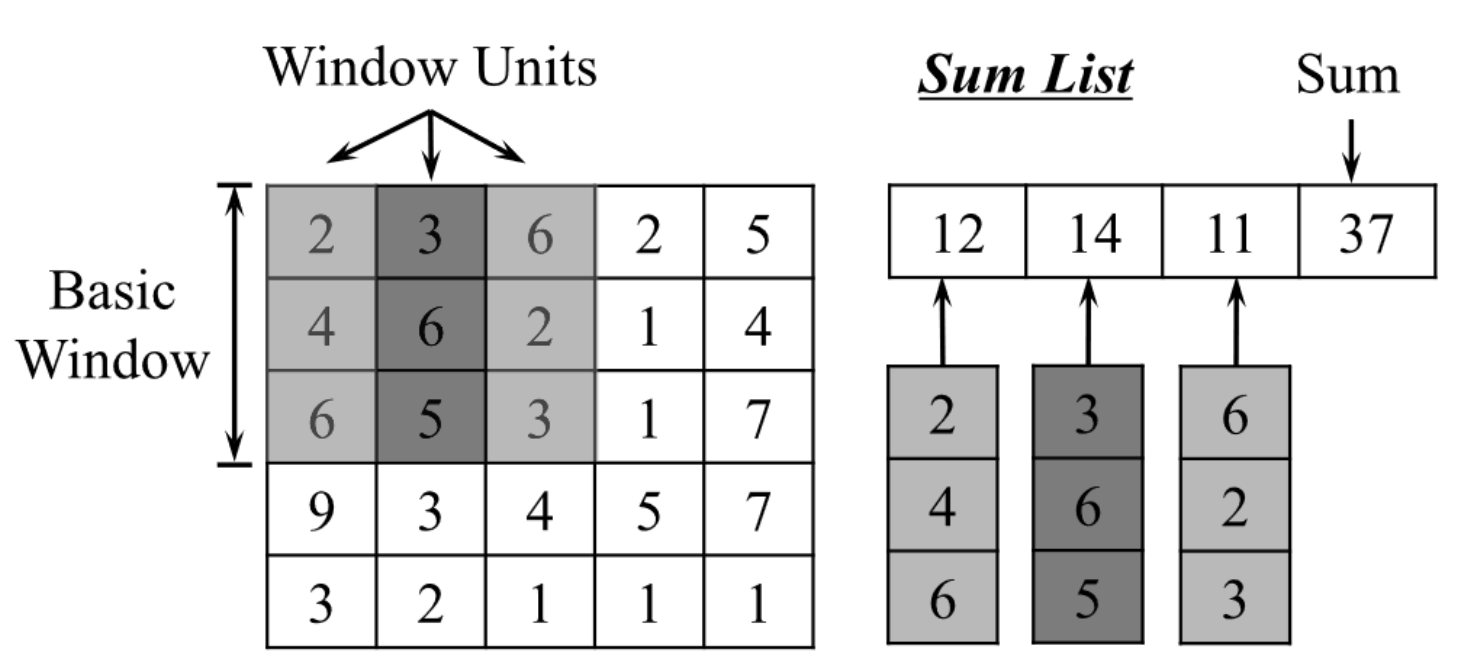
\includegraphics[width=0.7\textwidth]{windowAM_sum1.PNG}
\caption{Initialization of SUM window \cite{windowAggr}.}
\label{windowAM1}
\end{figure}

\begin{figure}
\centering
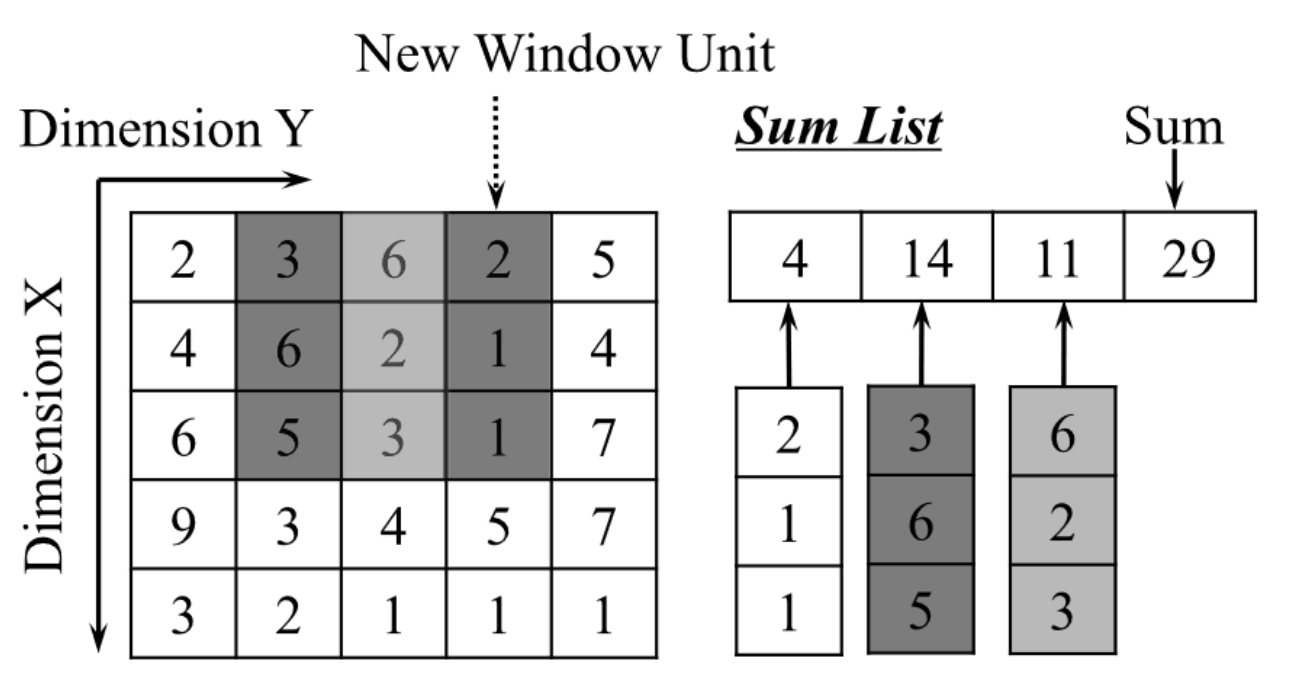
\includegraphics[width=0.63\textwidth]{windowAM_sum2.PNG}
\caption{Processing of a new unit and updating sum-list \cite{windowAggr}.}
\label{windowAM2}
\end{figure}

Min and max operators are handled by creating a heap data structure. The operator will generate basic window and scan window units in it and compute MIN/MAX for each one while inserting them into MIN/MAX heap. Then it moves the window along with the last dimension, obtains new window, calculates new MIN/MAX and insert it into MIN/MAX heap again. Finally it checks the heap root and removes it if its corresponding window unit is no longer present in the current window (this step is repeated until it corresponds). Proceed forward and calculate MIN of all windows derived while continuing to move the basic window down.

Percentile operator is a bit different from operators above. it is counted as $n=(P/100)*N+1/2$ and its structure is Self balancing binary search tree (SBST). Steps are: generate basic window, initialize SBST, insert all the values of the basic window into SBST, move the window forward along with the last dimension, insert new elements into SBST and delete old ones (i.e. ones not longer present in the current window). Then move forward and proceed to new basic window. \cite{windowAggr}


\section{Multidimensional Approximate Pattern Matching}\label{multidimApprPattMatch}
As was already stated in the problem specification \ref{spec} to successfully solve this problem, the user needs to specify certain pattern that will be searched for in the data. There are two options on how to look for the pattern i.e. with or without allowance of errors. According to this condition the problem is said to be approximate pattern matching when errors are allowed and exact vice versa.

Solution of this problem can be used in the field of text searching, pattern recognition or computational biology.

\subsection{Existing Solutions}

First and easiest approach is to compute the Edit distance between the pattern and data but it can be used only when the problem consists of one dimension and it computes exact pattern match. Another solution (this time for approximate match) can be performed by dynamic programming which tries to find all segments whose edit distance to pattern is maximally k, where k is greater than zero and lesser then complete match. This solution can be improved by filters.

When the problem consists of two dimensions there can be uses a variety of methods. Subset of this solutions works only for string data and the main algorithms were developed by: Bird and Baker, Amir and Landau, Zhu and Takaoka, K{\"a}rkk{\"a}inen and Ukkonen.

Scientists Krithivasan and Sitalakshmi developed The KS model which given two images of the same size, the edit distance is the sum of the edit distance of the corresponding row images. When used for approximate matching the sub-image of size $MxM$ is searched into a large image of size $NxN$, where they are using a generalization of the classical one-dimensional algorithm.

When fast searching under the KS model \ref{ks} patterns and texts are rectangular. Special distance measure allows errors along rows but not along columns. Variations of this model are Exact Partitioning which is best for larger patterns, Superimposed Automata which is best for small patterns, Counting is best for small patterns and One error. There are two useful functions defined for this model. First of them is C(m,k,r) function which defines cost per text character to search r patterns of length m with k errors, and second is L(m,r) function that says the value for k/m where the one dimensional algorithm does not work any more.

Another option to solve this problem is R model where each row is treated as a single string which is compared to other rows using one dimensional algorithm. Whole rows can be inserted and deleted. Modification of this model is RC model. If this algorithms encounter more than two dimensional problem it can be functional only if it has two hypercubes to compare which are reasonably close in size.

When tasked with a string pattern matching, various methods can be used for improving of the comparisons time, like for example Knuth--Morris--Pratt algorithm described in the section \ref{KMP}.

\subsection{Multidimensional Pattern Matching Algorithms}
To search across multiple dimension there are various algorithms to use, four of them are mentioned here. 

First of them is Exact Multidimensional Pattern Matching which divides the space along one dimension to obtain patterns of one dimension less. Then it searches all sub-patterns in each of the dimensional subtexts.

Second one is Fast filter for multidimensional approximate searching. This algorithm splits pattern across every dimension and then it searches sub-patterns the same way as exact solution, but all solutions found are checked by using the dynamic programming. 

Third is A stricter filter which says that whenever a piece appears the neighborhood can be checked. Its phase of finding possible solution positions is the same as in the previous algorithm but before checking the neighborhood with the use of dynamic programming the phase known as \textit{preverification} happens, in this phase all pieces of the pattern are checked one by one to see if they match where they should and only when finding sufficient number of pieces (i.e. size of the pattern minus errors that can happen along every dimension) that fit exactly then dynamic check can happen. 

Last algorithm presented is focused on adapting the filter to simpler distances. \cite{mdApproxPM}

These algorithms were not implemented by anyone yet, but I will provide detailed description of my solutions in section Implementation.

\subsection{Knuth--Morris--Pratt Algorithm}\label{KMP}
This algorithm was first presented in 1977 by scientists Knuth, Morris and Pratt \cite{kmp}. In their work they describe new algorithm usable for a string searching. The main idea of it is to remember for each position of the pattern P the length of the longest suffix P which matches to the prefix of the P. unlike the naive algorithm that after every mismatch shifts only by one position, which causes some parts of the data to be read again, KMP notices that it is possible to 
move by more than one position, this information is gained when comparing previous characters. To be able to remember all the extra information the algorithm uses is stored in a pre-computed table.

\begin{figure}
\centering
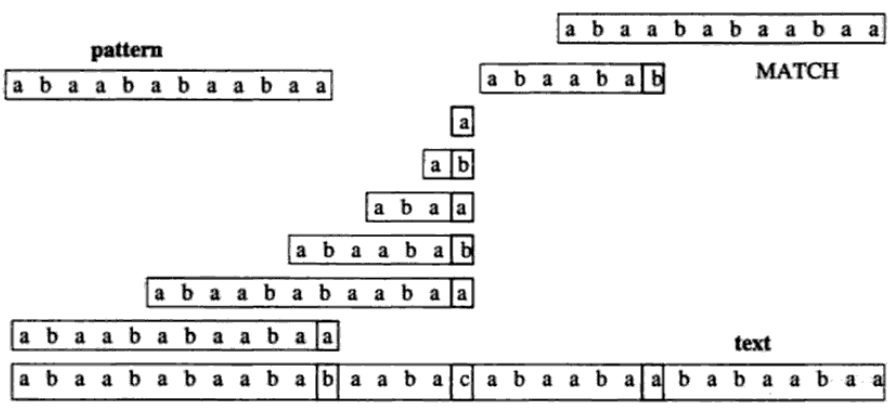
\includegraphics[scale=0.4]{KMP}
\caption{Example of matching of KMP algorithm \cite{stringJewels}. }
\end{figure}

\section{Machine Learning Based Methods}\label{machineLearning}
Main use of Machine Learning methods is in situations when in need of data analysis because people can often make mistakes, which make it difficult to find certain solutions.
These methods can be successfully applied in these situations and improve both the system efficiency and machine design. 

By working with the same set of features (here attributes) these algorithms can be even used when trying discover new data dependencies, classes and patterns. \cite{mlbm}
\subsection{KNN}
KNN or k Nearest Neighbors algorithm is very simple method of classifying items based on their distance to the pattern. The main goal of this procedure is to find \textit{k} nearest neighbors to the wanted item and classify it by the major class of its neighbors. This method is widely used since the 1970 and its one of the first and effective methods used for data mining.

First KNN algorithm was based on the Euclidean distance between the items, but it is possible to use other similarity measures (i.e they must meet the 4 basic criteria). Among the most widely used metrics belong: Euclidean distance, Kullback-Leibler distance, chess distance, Manhattan distance and Minkowski distance.

This approach is also known as similarity search, proximity search or close item search. Alternative way is introduced in \textit{R}-near neighbor search which is using a fixed radius. This algorithm tries to find all items that are within the distance \textit{R}. \cite{hashing}

One of the usable methods for solving this problem is using the Locality Sensitive Hashing.

\subsection{Kernel based methods}
Most of the machine learning based algorithms was developed for the usage in linear spaces while real word data often require nonlinear methods for dependency detection. By using kernel methods the dimensionality of the space can be reduced to a dot product. In this case the product acts as a similarity function between the pairs of data. The existence of a product like this enables these methods to act without computing the coordinates of the data but only computing the similarity between all of their pairs. Another advantage is that it is usually cheap to compute.

Among the algorithms using this method belong Support Vector Machines, Principal Component Analysis, Ridge regression, Linear Adaptive Filters and others. All linear models can be changed into non-linear by using kernel functions instead of its predictors. \cite{kernel} \cite{machineLearning}

All of these methods can be converted to work when using array data structure as mentioned in this paper \cite{kernelArray}. Also this paper \cite{kernelstring} explains how to define kernels on structured objects like strings. The main idea is to define a kernel between parts of the object by using a suitable similarity measure. Because of this, the kernel function can be designed even for graphs.

\section{Similarity join}
This join can be used on array data model which means a model where multidimensional array is defined by a set of dimensions and a set of attributes. Each dimension is a finite totally ordered discrete set and all cells in a given array have the same type. It must allow chunking and have shared-nothing architecture. Array join is a join of dimensions and union of attributes. The goal of the similarity join is to find all the pairs of points such that the distance between them is smaller than some Epsilon.
When applied on arrays the result dimension is union of joined arrays dimensions, result cells are the ones satisfying the given condition ($k=j+l$ in the picture), this can handle arrays with various dimensionality. Most general algorithm used for this is nested loop join. \cite{simJoin}
\begin{figure}
\centering
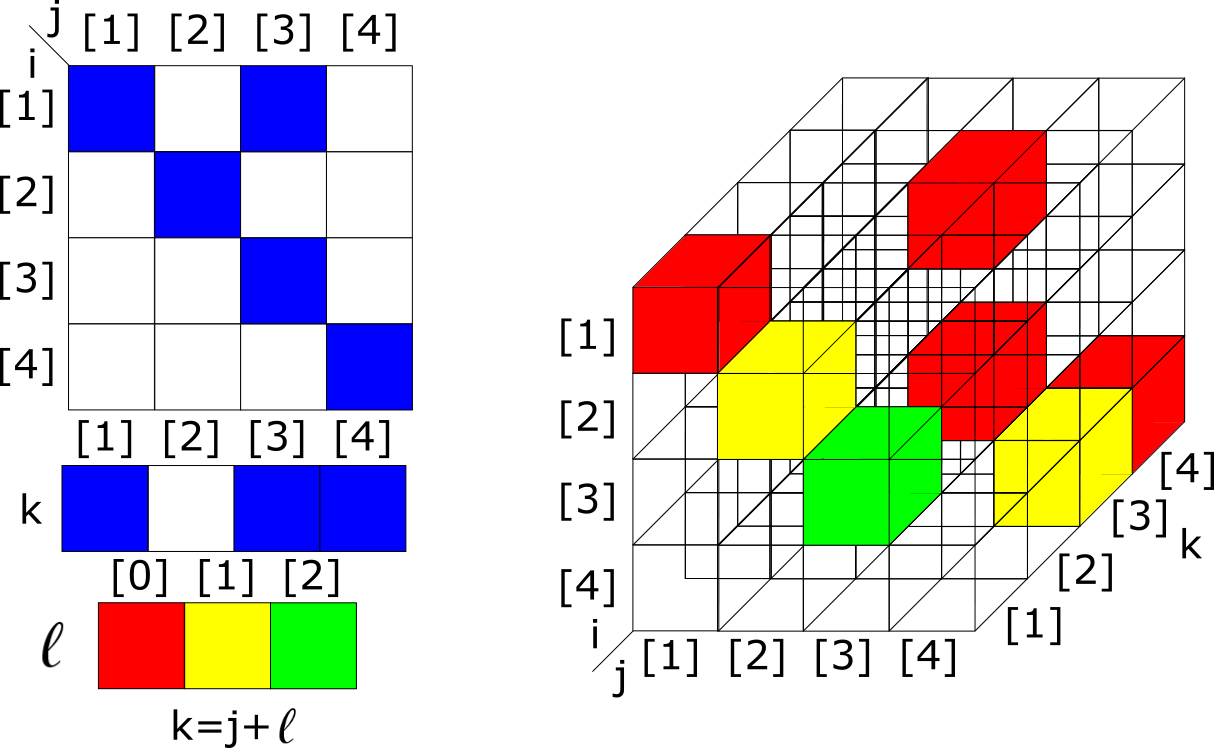
\includegraphics[scale=0.4]{simjoin.png}
\caption{Similarity join of 2 different arrays, first 2 dimensional, second 1 dimensional with condition array $\ell$. Result is in the 3 dimensional cube.}
\end{figure}


